\chapter{Eigenvalues, Eigenvectors and Diagonal Matrices}

\section{Eigenvalues and Eigenvectors}

\begin{definition}
    Let $\mat A$ be an $n \times n$ matrix. Let the non-zero vector $\vec x \in \RR^n$ be such that $\mat A \vec x$ is a scalar multiple of $\vec x$. That is, $\vec x$ satisfies the equation \[\mat A \vec x = \l \vec x\] for some scalar $\l$. The scalar $\l$ is an \vocab{eigenvector} of $\mat A$, and $\vec x$ is the \vocab{eigenvector} of $\mat A$ corresponding to $\l$.
\end{definition}

\subsection{Geometrical Interpretation}

Let $\vec x$ be an eigenvector of $\mat A$ with eigenvalue $\l$. Geometrically, this means $\mat A$ maps $\vec x$ along the same line through the origin as $\vec x$, but scaling it by a factor of $\l$. If $\l < 0$, the direction is reversed.

\begin{minipage}{0.33 \textwidth}
    \begin{figure}[H]\tikzsetnextfilename{446}
    \centering
    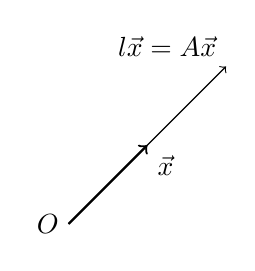
\begin{tikzpicture}
        \draw[black, thick, ->] (0, 0) -- (1, 1) node[anchor=north west] {$\vec x$};
        \draw[black, thin, ->] (0, 0) -- (2, 2) node[anchor=south east] {$\l \vec x = \mat A \vec x$};
        \node[anchor=east] (0, 0) {$O$};
    \end{tikzpicture}
    \caption{$\l > 1$}
    \end{figure}
\end{minipage}
\begin{minipage}{0.33 \textwidth}
    \begin{figure}[H]\tikzsetnextfilename{447}
    \centering
    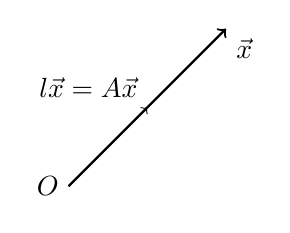
\begin{tikzpicture}
        \draw[black, thick, ->] (0, 0) -- (2, 2) node[anchor=north west] {$\vec x$};
        \draw[black, thin, ->] (0, 0) -- (1, 1) node[anchor=south east] {$\l \vec x = \mat A \vec x$};
        \node[anchor=east] (0, 0) {$O$};
    \end{tikzpicture}
    \caption{$0 \leq \l \leq 1$}
    \end{figure}
\end{minipage}
\begin{minipage}{0.33 \textwidth}
    \begin{figure}[H]\tikzsetnextfilename{448}
    \centering
    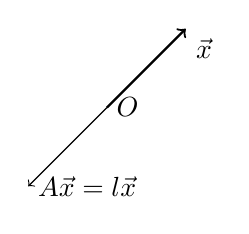
\begin{tikzpicture}
        \draw[black, thick, ->] (0, 0) -- (1, 1) node[anchor=north west] {$\vec x$};
        \draw[black, thin, ->] (0, 0) -- (-1, -1) node[anchor=west] {$\mat A \vec x = \l \vec x$};
        \node[anchor=west] (0, 0) {$O$};
    \end{tikzpicture}
    \caption{$\l < 0$}
    \end{figure}
\end{minipage}

\subsection{Finding Eigenvalues and Eigenvectors}

\begin{definition}
    The \vocab{characteristic polynomial} $\c(\l)$ of an $n \times n$ matrix $\mat A$ is the $n$ degree polynomial in $\l$ given by \[\c(\l) = \det{\mat A - \l \mat I}.\] The \vocab{characteristic equation} of $\mat A$ is \[\c(\l) = 0.\]
\end{definition}

\begin{proposition}
    $\l$ is an eigenvalue of $\mat A$ if and only if it satisfies the characteristic equation of $\mat A$.
\end{proposition}
\begin{proof}
    To find eigenvalues and eigenvectors, we must solve the equation $\mat A \vec x = \l \vec x$. Manipulating this equation, we see that \[\mat A \vec x - \l \vec x = \bp{\mat A - \l \mat I} \vec x = 0.\] Since $\vec x$ is non-zero, the null space of $\mat A - \l \mat I$ must be non-trivial. Thus, $\mat A - \l \mat I$ must be singular, so \[\c(\l) = \det{\mat A - \l \mat I} = 0.\] Thus, $\l$ satisfies the characteristic equation of $\mat A$.
\end{proof}

Since the characteristic equation can be easily solved, we now have a straightforward way of finding eigenvalues and eigenvectors.

\begin{recipe}[Finding Eigenvalues and Eigenvectors]
    We solve the characteristic equation $\c(\l) = \det{\mat A - \l \mat I} = 0$ to find possible eigenvalues $\l$. For each $\l$ found, we find its associated eigenvector(s) by finding the basis of the null space of $\mat A - \l \mat I$.
\end{recipe}

\begin{sample}
    Find the eigenvalues and eigenvectors of the matrix \[\mat A = \begin{pmatrix}1 & 2 \\ 5 & 4\end{pmatrix}.\]
\end{sample}
\begin{sample}
    The characteristic polynomial is \[\c(\l) = \det{\mat A - \l \mat I} = \det \begin{pmatrix}1 - \l & 2 \\ 5 & 4-\l\end{pmatrix} = \l^2 - 5\l -6 = (\l - 6)(\l + 1).\] Thus, the solutions to the characteristic equation $\c(\l) = 0$ are $\l = 6$ and $\l = -1$.

    Let $\vec x = \cveciix{x}{y}$ be a non-zero vector with $\mat A \vec x = \l \vec x.$

    \case{1}[$\l = 6$] We have \[\mat A - \l \mat I = \begin{pmatrix}-5 & 2 \\ 5 & -2\end{pmatrix} \cvecii{x}{y} = \cvecii00.\] Solving, we get $5x - 2y = 0$. Taking $x = 2$ and $y = 5$, the corresponding eigenvector is \[\vec x = \cvecii{2}{5}.\]

    \case{2}[$\l = -1$] We have \[\mat A- \l \mat I = \begin{pmatrix}2 & 2 \\ 5 & 5\end{pmatrix} \cvecii{x}{y} = \cvecii00.\] Solving, we get $x + y = 0$. Taking $x = 1$ and $y = -1$, the corresponding eigenvector is \[\vec x = \cvecii1{-1}.\]
\end{sample}

If $\mat A$ is a $3 \times 3$ matrix, we can use cross products to easily find eigenvectors.

\begin{sample}
    Let \[\mat A = \begin{pmatrix}2 & 0 & 1 \\ -1 & 2 & 3 \\ 1 & 0 & 2\end{pmatrix}.\] Find the eigenvector of $\mat A$ corresponding to $\l = 1$.
\end{sample}
\begin{sample}
    Let $\vec x$ be the desired eigenvector. Consider \[\bp{\mat A - \mat I} \vec x = \begin{pmatrix}1 & 0 & 1 \\ -1 & 1 & 3 \\ 1 & 0 & 1\end{pmatrix} \vec x = \cveciii000.\] By multiplying out the LHS, we get the following two equations: \[\vec x \dotp \cveciii101 = 0, \quad \vec x \dotp \cveciii{-1}13 = 0.\] These are precisely the equations of two planes, normal to $\cveciiix101$ and $\cveciiix{-1}13$ respectively, that also pass through the origin. Thus, $\vec x$ lies on the line of intersection between the two planes. The direction vector of this line is given by the cross product of the two normal vectors, so \[\vec x = \cveciii101 \crossp \cveciii{-1}13 = \cveciii{-1}{-4}1.\]
\end{sample}

Note that an $n \times n$ matrix may have less than $n$ eigenvalues and eigenvectors. For instance, \[\begin{pmatrix}3 & 1 \\ 0 & 3\end{pmatrix}\] has the sole eigenvalue $\l = 3$ with corresponding eigenvector $\cveciix10$.

Also, one eigenvalue may have multiple corresponding eigenvectors. For instance, \[\begin{pmatrix}0 & 0 & -2 \\ 1 & 2 & 1 \\ 1 & 0 & 3\end{pmatrix}\] has eigenvalue $\l = 2$, which corresponds to two linearly independent eigenvectors: \[\vec x_1 = \cveciii{-1}01, \quad \vec x_2 = \cveciii010.\]

\subsection{Useful Results}

\begin{proposition}
    Eigenvectors corresponding to distinct eigenvalues must be linearly independent.
\end{proposition}
\begin{proof}
    By way of contradiction, suppose the eigenvectors are linearly dependent. Let $j$ be the maximal $j$ such that $\vec x_1, \dots, \vec x_j$ are linearly independent. Then $\vec x_{j+1}$ can be expressed as a linear combination of $\vec x_1, \dots, \vec x_j$: \[\vec x_{j+1} = a_1 \vec x_1 + \dots + a_j \vec x_j. \tag{1}\] Applying $\mat A$ on both sides, we see that \[\l_{j+1} \vec x_{j+1} = a_1 \l_1 \vec x_1 + \dots + a_j \l_j \vec x_j.\tag{2}\] Since $\vec x_1, \dots, \vec x_j$ are linearly independent, we can compare their coefficients in (1) and (2), which gives \[a_i = a_i \frac{\l_i}{\l_{j+1}} \implies \l_i = \l_{j+1}\] for all $1 \leq i \leq j$. But this clearly contradicts the supposition that the eigenvalues are distinct. Thus, the eigenvectors must be linearly independent.
\end{proof}

\begin{proposition}
    If $\mat A$ is a triangular matrix, then the eigenvalues of $\mat A$ are the entries on the principal diagonal of $\mat A$.
\end{proposition}
\begin{proof}
    Recall that the determinant of a triangular matrix is the product of its principal diagonal entries. Thus, \[\c(\l) = \det{\mat A - \l \mat I} = \bp{a_{11} - \l}\bp{\a_{22} - \l} \dots \bp{a_{nn} - \l},\] whence the roots are $\l = a_{11}, a_{22}, \dots, a_{nn}$.
\end{proof}

\begin{proposition}
    Suppose $\vec x$ is an eigenvector of an $n \times n$ matrix $\mat A$ with corresponding eigenvalue $\l$.
    \begin{enumerate}
        \item For any real number $k$, $\vec x$ is an eigenvector of the matrix $k \mat A$, with corresponding eigenvalue $k \l$.
        \item For any positive integer $m$, $\vec x$ is an eigenvector of the matrix $\mat A^m$, with corresponding eigenvalue $\l^m$.
        \item If $\mat A$ is invertible, then $\vec x$ is an eigenvector of $\mat A^{-1}$ with corresponding eigenvalue $\l^{-1}$ when $\l \neq 0$.
        \item If $\vec x$ is also an eigenvector of an $n \times n$ matrix $\vec B$ with corresponding eigenvalue $\m$, then $\vec x$ is an eigenvector of the sum $\mat A + \mat B$, with corresponding eigenvalue $\l + \m$.
    \end{enumerate}
\end{proposition}
\begin{proof}[Proof of \emph{(a)}]
    Since $\mat A = \l \vec x$, we have $\bp{k \mat A} \vec x = \bp{k \l} \vec x$.
\end{proof}
\begin{proof}[Proof of \emph{(b)}]
    We use induction. Let the statement $P(m)$ be such that \[P(m) \iff \text{$\vec x$ is an eigenvector of the matrix $\mat A^m$ with corresponding eigenvalue $\l^m$}.\] The base case $m = 1$ is trivial. Suppose $P(k)$ is true for some $k \in \NN$. Then \[\mat A^{k+1} \vec x = \mat A \bp{\mat A^k \vec x} = \mat A \bp{\l^k \vec x} = \l^k \bp{\mat A \vec x} = \l^k \bp{\l \vec x} = \l^{k+1} \vec x.\] Thus, $P(k) \implies P(k+1)$. This closes the induction.
\end{proof}
\begin{proof}[Proof of \emph{(c)}]
    Since $\mat A = \l \vec x$, we have \[\vec x = \mat A^{-1} \mat A \vec x = \mat A^{-1} \l \vec x = \l \bp{\mat A^{-1} \vec x} \implies \mat A^{-1} \vec x = \l^{-1} \vec x.\]
\end{proof}
\begin{proof}[Proof of \emph{(d)}]
    Since $\mat A = \l \vec x$ and $\mat B = \m \vec x$, we have \[\bp{\mat A + \mat B} \vec x = \mat A \vec x + \mat B \vec x = \l \vec x + \m \vec x = \bp{\l + \m} \vec x.\]
\end{proof}

\begin{corollary}
    Let $\vec x$ be an eigenvector of $\mat A$ with corresponding eigenvalue $\l$. Define a polynomial $p(X) = a_0 + a_1 X + a_2 X^2 + \dots + a_n X^n$. Then $p(\l) \vec x = p(\mat A) \vec x$.
\end{corollary}
Note that we are taking $a_0$ to mean $a_0 \mat I$ on the RHS.

\begin{definition}
    A \emph{submatrix} of $\mat A$ is a matrix obtained from $\mat A$ by deleting a collection of rows and/or columns. A \emph{principal submatrix} of $\mat A$ is a submatrix whereby the indices of the deleted rows are the same as the indices of the deleted columns. A \emph{principal minor} of order $k$ is the determinant of a $k \times k$ principal submatrix.
\end{definition}

\begin{example}
    Given \[\mat A = \begin{pmatrix}1 & 2 & 3 \\ 4 & 5 & 6 \\ 7 & 8 & 9\end{pmatrix},\] the following three matrices are submatrices of $\mat A$: \[\mat B_1 = \begin{pmatrix}1 & 2 \\ 4 & 5\end{pmatrix}, \quad \mat B_2 = \begin{pmatrix}4 & 6 \\ 7 & 9\end{pmatrix}.\] To obtain $\mat B_1$, we deleted the third row and third column. To obtain $\mat B_2$, we deleted the first row and second column. Note that $\mat B_1$ is also a principal submatrix.
\end{example}

\begin{proposition}
    Let $\mat A$ be an $n \times n$ matrix. Let $E_k$ be the sum of the determinants of all principal minors of order $k$. We define $E_0 = 1$. Then the characteristic polynomial $\c(\l)$ of $\mat A$ is given by \[\c(\l) = \sum_{i = 0}^n (-1)^i E_{n-i} \l^i.\]
\end{proposition}

For a proof, see this \href{https://boonsuan.github.io/misc/cauchy_binet.pdf}{wonderful note} by Ho Boon Suan.

\begin{example}
    Consider \[\mat A = \begin{pmatrix}2 & 0 & 1 \\ -1 & 2 & 3 \\ 1 & 0 & 2\end{pmatrix}.\] Then
    \begin{align*}
        E_1 &= \abs{2} + \abs{2} + \abs{2} = 6,\\
        E_2 &= \begin{vmatrix}2 & 0 \\ -1 & 2\end{vmatrix} + \begin{vmatrix}2 & 3 \\ 0 & 2\end{vmatrix} + \begin{vmatrix}2 & 1 \\ 1 & 2\end{vmatrix} = 11,\\
        E_3 &= \begin{vmatrix}2 & 0 & 1 \\ -1 & 2 & 3 \\ 1 & 0 & 2\end{vmatrix} = 6.
    \end{align*}
    Invoking the above result, we see that \[\c(\l) = -\l^3 + E_1 \l^2 - E_2 \l + E_3 = -\l^3 + 6 \l^2 - 11 \l + 6.\]
\end{example}

\begin{corollary}
    If $\mat A$ is an $n \times n$ matrix,
    \begin{itemize}
        \item The sum of the $n$ eigenvalues of $\mat A$ (counting multiplicity) is equal to the trace of $\mat A$.
        \item The product of the $n$ eigenvalues of $\mat A$ (counting multiplicity) is equal to the determinant of $\mat A$.
    \end{itemize}
\end{corollary}
\begin{proof}
    Apply Vieta's formula to the above result.
\end{proof}

\section{Diagonal Matrices}

Recall that a diagonal matrix $\mat D$ is a square matrix where all off-diagonal entries are zero. Diagonal matrices have nice properties that make computations involving them simple and convenient:
\begin{itemize}
    \item $\det \mat D$ is the product of its diagonal entries.
    \item If $\det \mat D \neq 0$, then $\mat D^{-1}$ is a diagonal matrix with the corresponding reciprocals in the diagonal.
    \item $\mat D^{n}$ is a diagonal matrix with the corresponding powers in the diagonal.
\end{itemize}
For instance, if \[\mat D = \begin{pmatrix}1 & 0 & 0 \\ 0 & 2 & 0 \\ 0 & 0 & 3\end{pmatrix},\] then \[\mat D^{100} = \begin{pmatrix}1^{100} & 0 & 0 \\ 0 & 2^{100} & 0 \\ 0 & 0 & 3^{100}\end{pmatrix} \quad \tand \quad \mat D^{-100} = \begin{pmatrix}1^{-100} & 0 & 0 \\ 0 & 2^{-100} & 0 \\ 0 & 0 & 3^{-100}\end{pmatrix}.\]

\subsection{Diagonalization}

The useful properties of diagonal matrices motivates us to find a way to write an $n \times n$ matrix in terms of a diagonal matrix, i.e. diagonalize $\mat A$ in some way.

\begin{definition}
    A matrix $\mat A$ is \vocab{diagonalizable} if there exists an invertible matrix $\mat Q$ such that $\mat A = \mat Q \mat D \mat Q^{-1}$, where $\mat D$ is a diagonal matrix. We say that $\mat Q$ \vocab{diagonalizes} $\mat A$.
\end{definition}

\begin{proposition}
    If $\mat A$ is diagonalizable, then the columns of $\mat Q$ are the linearly independent eigenvectors of $\mat A$, and the diagonal matrix $\mat D$ contains the corresponding eigenvalues.
\end{proposition}
\begin{proof}
    Let $\mat A$ be an $n \times n$ matrix with eigenvectors $\vec x_1, \dots, \vec x_n$ corresponding to the real eigenvalues $\l_1, \dots, \l_n$. Let $\mat Q$ be the matrix with $\vec x_1, \dots, \vec x_n$ as its columns and let $\mat D$ be a diagonal matrix with its diagonal entries as $\l_1, \dots, \l_n$: \[\mat Q = \begin{pmatrix}\vec x_1 & \dots & \vec x_n\end{pmatrix}, \quad \mat D = \begin{pmatrix}\l_1 & \dots & 0 \\ \vdots & \ddots & \vdots \\ 0 & \dots & \l_n\end{pmatrix}.\] Then \[\mat A \mat Q = \begin{pmatrix}\mat A \vec x_1 & \dots & \mat A \vec x_n\end{pmatrix} = \begin{pmatrix}\l_1 \vec x_1 & \dots & \l_n \vec x_n\end{pmatrix} = \begin{pmatrix}\vec x_1 & \dots & \vec x_n\end{pmatrix} \begin{pmatrix}\l_1 & \dots & 0 \\ \vdots & \ddots & \vdots \\ 0 & \dots & \l_n\end{pmatrix} = \mat Q \mat D.\] Post-multiplying both sides by $\mat Q^{-1}$, which exists since the columns of $\mat Q$ are linearly independent, we have $\mat A = \mat Q \mat D \mat Q^{-1}$.
\end{proof}

Note that if $\mat A$ has $n$ real and distinct eigenvalues, it will have $n$ linearly independent eigenvectors, so it will be diagonalizable. However, if it has repeated eigenvalues, it may not be diagonalizable.

\begin{sample}
    Let \[\mat A = \begin{pmatrix}2 & 0 & 1 \\ -1 & 2 & 3 \\ 1 & 0 & 2\end{pmatrix}.\] Find a matrix $\mat Q$ and a diagonal matrix $\mat D$ such that $\mat A = \mat Q \mat D \mat Q^{-1}$.
\end{sample}
\begin{sampans}
    We previously found the corresponding eigenvectors for eigenvalues 1, 2, 3 to be \[\cveciii14{-1}, \quad \cveciii010, \quad \cveciii121.\] Thus, \[\mat Q = \begin{pmatrix}1 & 0 & 1 \\ 4 & 1 & 2 \\ -1 & 0 & 1\end{pmatrix} \quad \tand \quad \mat D = \begin{pmatrix}1 & 0 & 0 \\ 0 & 2 & 0 \\ 0 & 0 & 3 \end{pmatrix}.\]
\end{sampans}

Note that $\mat Q$ and $\mat D$ are not unique. Using the above sample problem, we could have taken \[\mat Q = \begin{pmatrix}1 & 1 & 0 \\ 2 & 4 & 1 \\ 1 & -1 & 0\end{pmatrix} \quad \tand \quad \mat D = \begin{pmatrix}3 & 0 & 0 \\ 0 & 1 & 0 \\ 0 & 0 & 2\end{pmatrix}.\]

\subsection{Computing Matrix Powers}

One of the more useful purposes of diagonalization is to compute matrix powers.

\begin{proposition}
    Suppose $\mat A = \mat Q \mat D \mat Q^{-1}$ is diagonalizable. Then \[\mat A^k = \mat Q \mat D^k \mat Q^{-1}.\]
\end{proposition}
\begin{proof}
    Observe that
    \begin{gather*}
        \mat A^k = \bp{\mat Q \mat D \mat Q^{-1}}\bp{\mat Q \mat D \mat Q^{-1}}\dots\bp{\mat Q \mat D \mat Q^{-1}} = \mat Q \mat D \bp{\mat Q^{-1} \mat Q} \mat D \bp{\mat Q^{-1} \mat Q} \dots \mat D \mat Q^{-1}\\
        = \mat Q \mat D \mat D \dots \mat D \mat Q^{-1} = \mat Q \mat D^{k} \mat Q^{-1}.
    \end{gather*}
\end{proof}

\begin{sample}
    Let \[\mat A = \begin{pmatrix}2 & 0 & 1 \\ -1 & 2 & 3 \\ 1 & 0 & 2\end{pmatrix}.\] Compute $\mat A^{10}$.
\end{sample}
\begin{sampans}
    We previously found that $\mat A = \mat Q \mat D \mat Q^{-1}$, where \[\mat Q = \begin{pmatrix}1 & 0 & 1 \\ 4 & 1 & 2 \\ -1 & 0 & 1\end{pmatrix} \quad \tand \quad \mat D = \begin{pmatrix}1 & 0 & 0 \\ 0 & 2 & 0 \\ 0 & 0 & 3 \end{pmatrix}.\] Thus, \[\mat A^{10} = \mat Q \mat D^{10} \mat Q^{-1} = \begin{pmatrix}1 & 0 & 1 \\ 4 & 1 & 2 \\ -1 & 0 & 1\end{pmatrix} \begin{pmatrix}1^{10} & 0 & 0 \\ 0 & 2^{10} & 0 \\ 0 & 0 & 3^{10} \end{pmatrix} \begin{pmatrix}1 & 0 & 1 \\ 4 & 1 & 2 \\ -1 & 0 & 1\end{pmatrix}^{-1},\] which evaluates to \[\mat A^{10} = \begin{pmatrix}29525 & 0 & 29524 \\ 55979 & 1024 & 60071 \\ 29524 & 0 & 29525\end{pmatrix}.\]
\end{sampans}